\chapter{Release 2 : Planification Locale et Consolidation Groupe (Sprints 2 et 3)}
\label{chap:sprints_2_3}

\section{Introduction}
Une fois le socle technique et les mécanismes de sécurité validés lors du Sprint 1, l'équipe projet a pu se consacrer au développement du cœur métier de \textit{Cofat Capacity Study}. Cette Release 2, subdivisée en deux Sprints majeurs (Sprint 2 et Sprint 3), constitue la véritable rupture technologique pour les employés du groupe. Dans un premier temps, le Sprint 2 vise à outiller les responsables d'usines (Site Managers) en remplaçant leurs processus manuels par des modules digitaux de planification locale des Équipements, des Espaces et des Ressources Humaines. Nous y détaillerons notamment l'algorithme robuste d'importation de fichiers Excel. Dans un second temps, le Sprint 3 exploite l'architecture centralisée de la base de données pour générer, à la volée, les consolidations à l'échelle mondiale de ces mêmes entités (Cofat Group). Ce chapitre abordera enfin la mise en place du référentiel \textit{StandardInvestment V2}, outil décisif pour l'évaluation des futurs investissements industriels du Groupe COFAT.

\section{Sprint 2 : Déploiement des modules de Planification Locale}
La planification locale est l'action par laquelle chaque usine projette ses besoins capacitaires en fonction des commandes automobiles à venir. L'objectif de ce sprint était de numériser cette étape de manière transparente, en conservant la souplesse d'Excel tout en apportant la rigueur d'une base de données relationnelle.

\subsection{Le Module des Équipements Industriels}
L'objectif du module "Équipements" est de permettre au Site Manager de suivre l'état de saturation de son parc de machines (presses, coupeuses, soudeuses) et d'identifier rapidement les goulots d'étranglement qui pourraient bloquer la production d'un nouveau projet automobile.

Avant l'interface, le Site Manager calcule théoriquement le besoin. Il le saisit ensuite dans l'application ou l'importe (nous verrons l'import plus bas).

\vspace{0.5cm}
\begin{figure}[H]
    \centering
    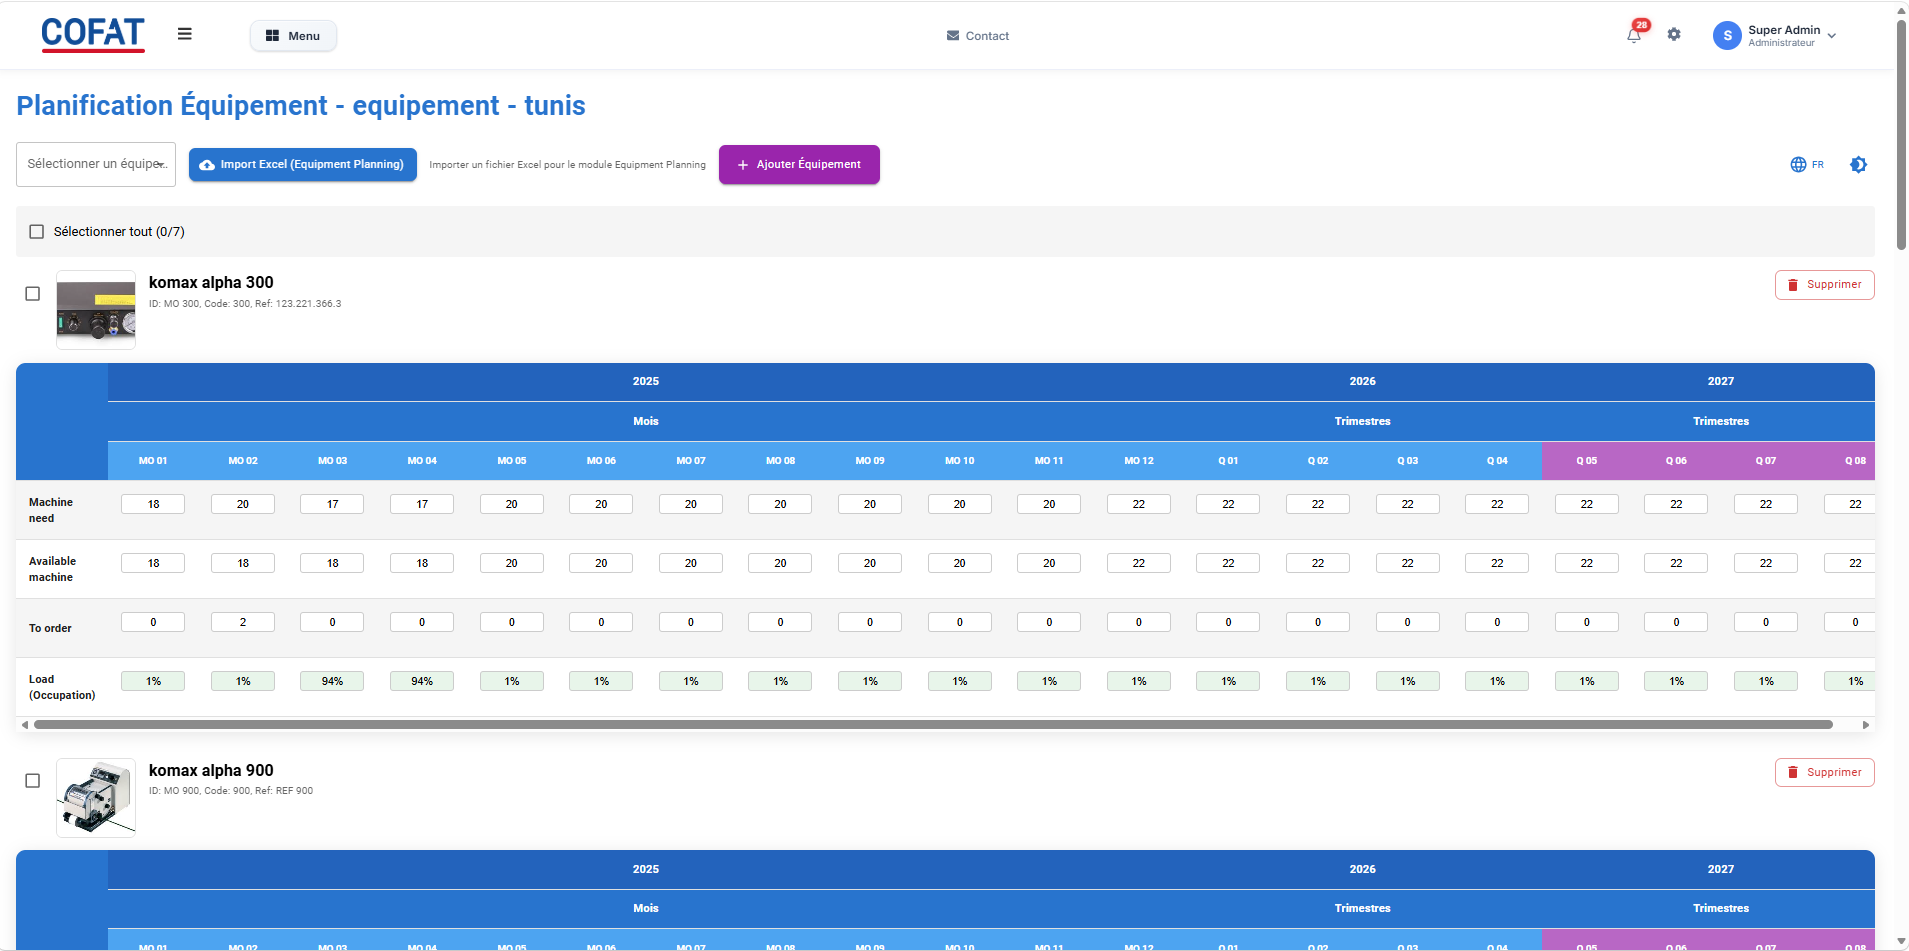
\includegraphics[width=1\textwidth]{img/planification equipement standard.png}
    \caption{Interface de planification locale des équipements}
    \label{fig:planif_equipement}
\end{figure}
\vspace{0.5cm}

\textbf{Analyse détaillée de l'interface (Figure \ref{fig:planif_equipement}) :}
La conception de cette interface a privilégié la clarté visuelle, car l'ingénieur méthodes doit scanner des dizaines de lignes en un clin d'œil. Le tableau de données, implémenté avec Material UI (DataGrid), présente les colonnes suivantes :
\begin{itemize}
    \item \textbf{Type d'Équipement} : La désignation de la machine (ex: Komax Alpha 530).
    \item \textbf{Opération} : L'application permet un filtrage dynamique par étape de production. L'utilisateur peut isoler les machines de la zone "1-COUPE", "2-PREPARATION", "3-ASSEMBLAGE" ou "4-CONTROLE ELECTRIQUE ET CONDITIONNEMENT".
    \item \textbf{machineNeed} : Le besoin calculé par l'ingénieur (par exemple 4.5 machines requises pour absorber le volume).
    \item \textbf{availableMachine} : Le parc physique réel sur le site (par exemple 4 machines).
    \item \textbf{load (\%)} : C'est le taux de charge, métrique fondamentale. Il est calculé algorithmiquement par le frontend React (et vérifié par le backend) selon la formule $Load = (machineNeed / availableMachine) \times 100$. Un code couleur visuel (conditional formatting) alerte immédiatement l'ingénieur :
        \begin{itemize}
            \item \textbf{Vert (Load $\le$ 80\%)} : Sous-charge, l'usine a de la marge.
            \item \textbf{Orange (80\% $<$ Load $\le$ 100\%)} : Zone de tension, l'équipement est optimisé au maximum.
            \item \textbf{Rouge (Load $>$ 100\%)} : Surcharge critique. Dans notre exemple (4.5 / 4), le load de 112.5\% s'affiche en rouge vif.
        \end{itemize}
    \item \textbf{toOrder} : Ce champ calcule le déficit. Si le load dépasse 100\%, il indique le nombre d'unités manquantes (ici 0.5, arrondi au supérieur pour la commande).
\end{itemize}

\subsection{Le Module d'analyse de l'Occupation des Espaces}
L'espace physique (surface au sol en m²) est une contrainte dure dans une usine de câblage. Une ligne d'assemblage ne peut pas être superposée. Le module "Espaces" permet d'avoir une vision cartographiée et quantitative de la surface disponible pour accueillir de futurs projets.

\vspace{0.5cm}
\begin{figure}[H]
    \centering
    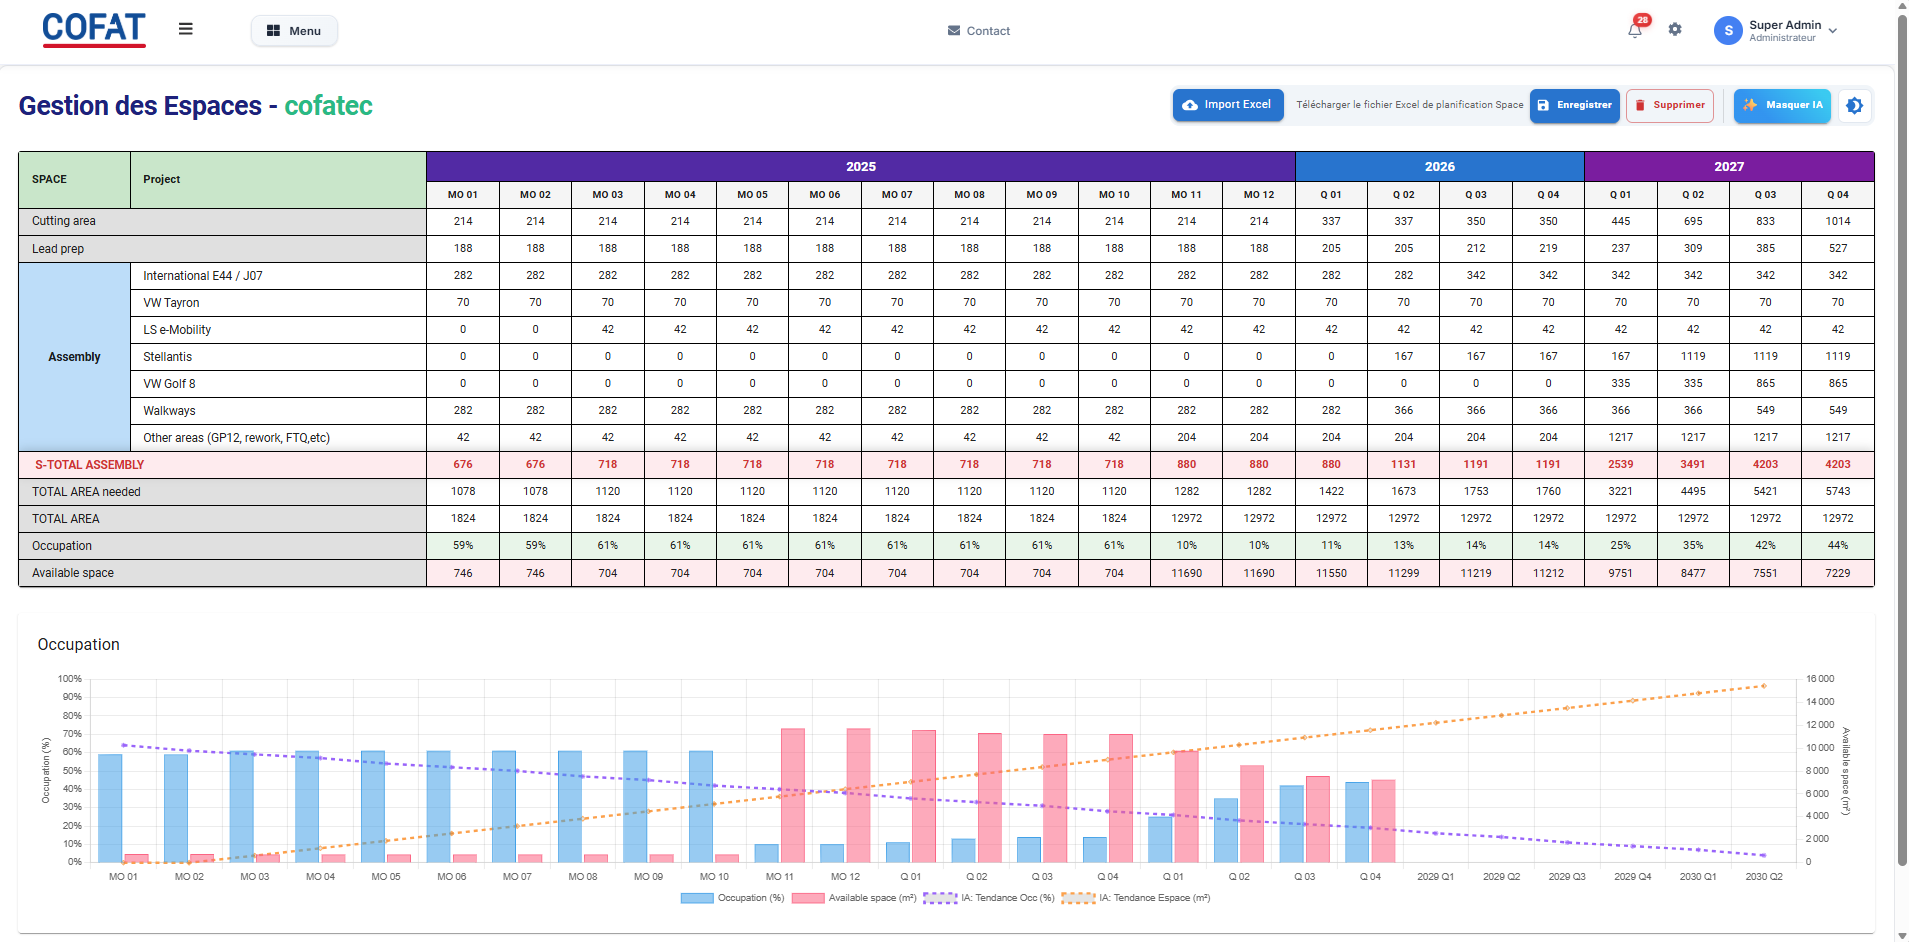
\includegraphics[width=0.9\textwidth]{img/analyse des espaces.png}
    \caption{Tableau de gestion des surfaces par zone de production}
    \label{fig:tableau_espaces}
\end{figure}
\vspace{0.5cm}

\vspace{0.5cm}
\begin{figure}[H]
    \centering
    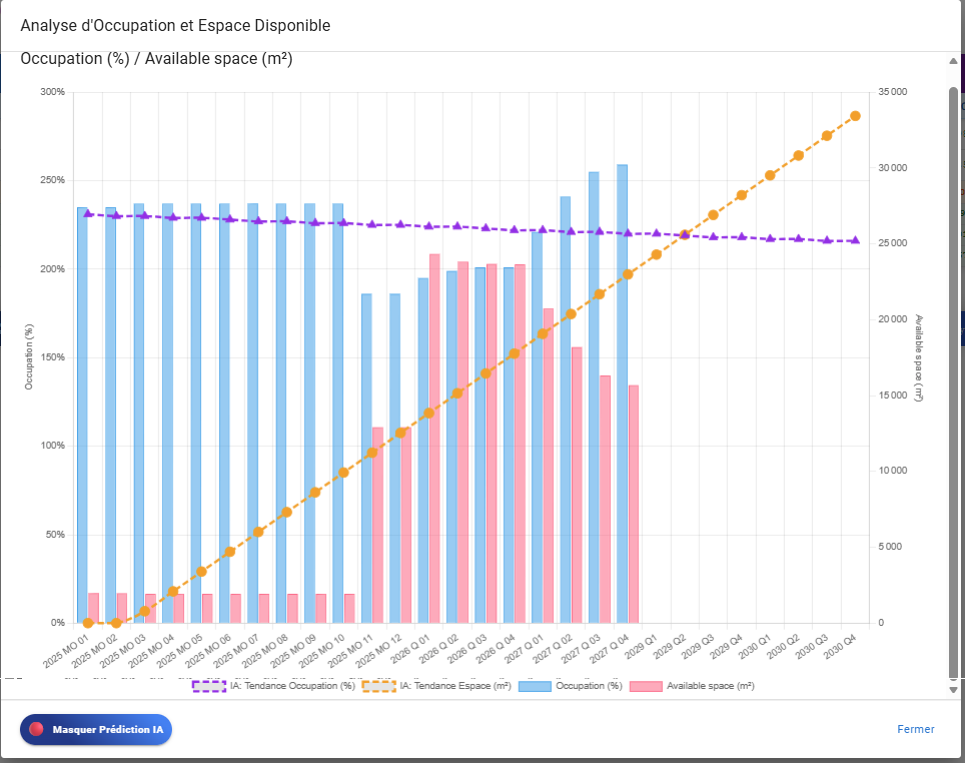
\includegraphics[width=0.9\textwidth]{img/analyse d'occupation et espace disponible.png}
    \caption{Tableau de bord visuel : Taux d'occupation global du site}
    \label{fig:graphique_espaces}
\end{figure}
\vspace{0.5cm}

\textbf{Analyse du fonctionnement du module Espaces :}
Comme illustré dans la Figure \ref{fig:tableau_espaces}, l'interface sépare l'usine en grandes zones logiques. On y retrouve les zones de traitement primaire (\textit{coupe}, \textit{préparation}) et les vastes halls dédiés aux projets clients majeurs (visibles dans l'interface : \textit{VW Tayron}, \textit{International E44}, \textit{Stellantis J4U}, \textit{VW Golf 8}, \textit{LS e-mobility BEV-A}). 

Pour chaque zone, l'ingénieur déclare la surface totale et la surface occupée. La Figure \ref{fig:graphique_espaces} met en évidence la puissance de la bibliothèque \textit{Charts.js}. Le composant React extrait ces données et génère un diagramme circulaire (Pie Chart) montrant, d'un coup d'œil, le ratio Espace Occupé / Espace Libre pour l'usine entière. Ce graphique interactif aide le directeur de site à décider rapidement s'il peut accepter la ligne de production d'un nouveau modèle de véhicule ou s'il doit louer une extension de bâtiment.

\subsection{Le Module de prévision des Ressources Humaines (RH)}
Le recrutement et la formation des opérateurs prennent des semaines. Le module RH permet d'anticiper les embauches sur un horizon de trois ans, répartis par catégories et par projets de véhicules.

\vspace{0.5cm}
\begin{figure}[H]
    \centering
    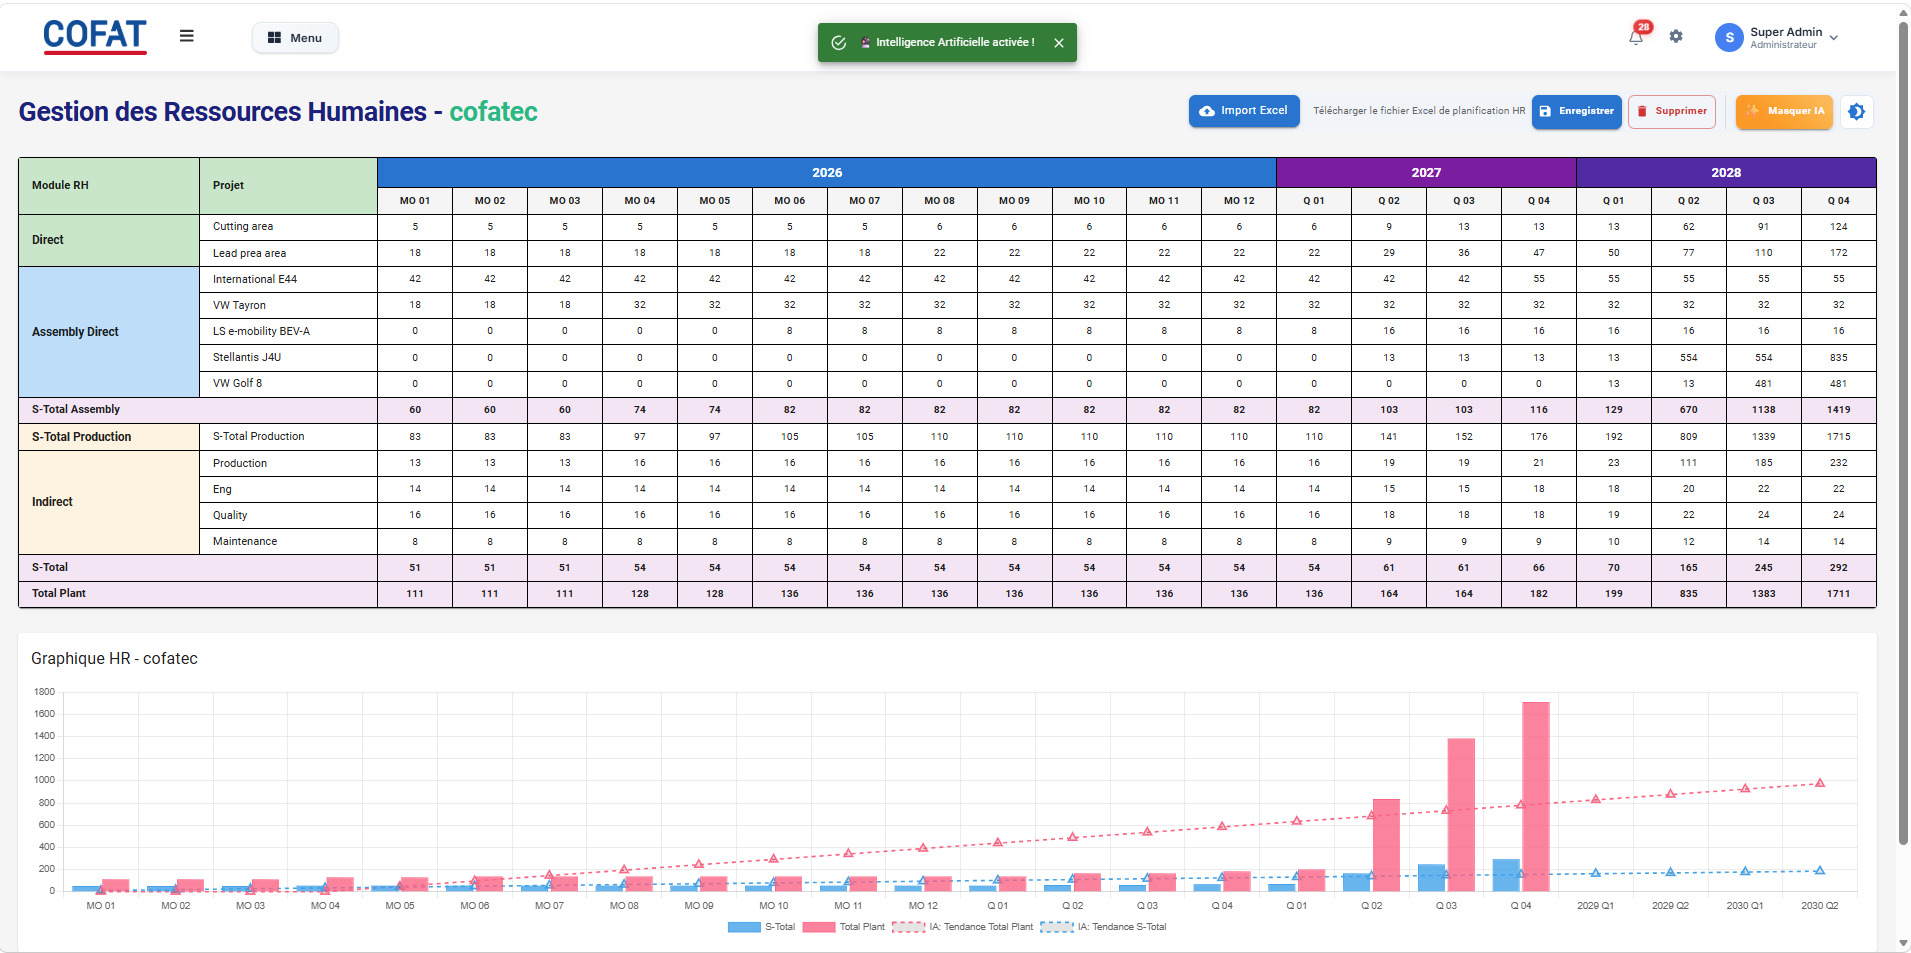
\includegraphics[width=1\textwidth]{img/gestion des resources humaines.png}
    \caption{Interface de planification temporelle des Ressources Humaines}
    \label{fig:planif_rh}
\end{figure}
\vspace{0.5cm}

\textbf{Analyse de la matrice temporelle RH (Figure \ref{fig:planif_rh}) :}
Ce module a été le plus complexe à modéliser ergonomiquement, car il présente une dimension temporelle très étendue. Le tableau de données, généré dynamiquement par un composant Ant Design, croise la dimension "Métier" avec la ligne de temps :
\begin{itemize}
    \item \textbf{Structuration en lignes} : Les effectifs sont regroupés par grandes catégories : \textit{Direct} (opérateurs machines), \textit{Indirect} (qualité, maintenance, logistique), et \textit{Assemblage Direct}. L'interface décline ensuite ces catégories par sous-projets (\textit{Cutting area}, \textit{Lead prea area}, et les projets d'assemblage comme \textit{VW Tayron} ou \textit{Stellantis J4U}).
    \item \textbf{Structuration en colonnes (Time-Series)} : Pour offrir une vision de \textit{ramp-up} (montée en cadence), le système affiche la prévision mensuelle pour l'année courante (colonnes MO 01 à MO 12 pour 2025), puis bascule sur une granularité trimestrielle pour les années futures (colonnes Q01 à Q04 pour 2026 et 2027).
\end{itemize}
Le système compare en permanence ces prévisions au \textit{Headcount} (effectif actuel) et calcule les écarts d'embauche.

\subsection{L'Ingénierie de l'Import Excel (Le cœur de la saisie de données)}
Saisir à la main des dizaines de cellules RH (12 mois + 8 trimestres par projet) dans un formulaire web aurait provoqué un rejet immédiat de l'application par les ingénieurs. C'est pourquoi j'ai développé un algorithme d'importation massive depuis des fichiers Excel (.xlsx).

\textbf{Le double processus technique réel (\textit{Hybrid Data Pipeline}) :}
L'application met en œuvre deux architectures d'importation distinctes selon le module, optimisant ainsi la répartition de charge réseau et la validation applicative :

\begin{enumerate}
    \item \textbf{Parsing Côté Client (Modules Équipements, RH, Espaces) :}
    \begin{itemize}
        \item \textbf{Lecture locale :} L'utilisateur sélectionne le fichier Excel localement. Le composant React (par exemple \texttt{ExcelImporterHR.js}) utilise l'API HTML5 \texttt{FileReader} pour charger le fichier dans un \texttt{ArrayBuffer} binaire en mémoire locale du navigateur, évitant ainsi un téléversement lourd et inutile sur le serveur.
        \item \textbf{Extraction et nettoyage :} La bibliothèque SheetJS (\texttt{xlsx}) instanciée côté client convertit le classeur en tableau d'objets JSON brut à l'aide de la méthode \texttt{XLSX.utils.sheet\_to\_json()}.
        \item \textbf{Validation dynamique :} Le code React valide la structure, isole les colonnes d'années, ignore les lignes vides, puis formate les lignes valides en un payload JSON structuré.
        \item \textbf{Envoi et persistance :} Ce tableau JSON est transmis par une simple requête HTTP \texttt{POST} (ex: \texttt{/api/hr/save}) au serveur Express, qui effectue un traitement de masse direct via la méthode \texttt{upsert} de Sequelize dans la base SQL Server.
    \end{itemize}
    \item \textbf{Parsing Côté Serveur (Module Budget Non-Industriel) :}
    \begin{itemize}
        \item \textbf{Téléversement (Multer) :} Le fichier Excel est envoyé sous forme de flux binaire multipart (\texttt{multipart/form-data}) vers le serveur. Le middleware \texttt{multer} réceptionne et enregistre le fichier de manière temporaire dans le dossier serveur \texttt{/Uploads/budget}.
        \item \textbf{Extraction serveur (XLSX) :} Le contrôleur Node.js prend le relais, ouvre le fichier avec \texttt{xlsx}, et parse la feuille correspondante en un tableau JSON.
        \item \textbf{Validation et Traitement :} Le serveur vérifie l'intégrité des lignes, recalcule les totaux, et insère les lignes valides en base de données. Enfin, le fichier temporaire est supprimé physiquement du disque serveur (\texttt{fs.unlinkSync()}) pour libérer l'espace.
    \end{itemize}
\end{enumerate}

\section{Sprint 3 : La Consolidation Mondiale (Cofat Group)}
Si la planification locale (Sprint 2) permet aux usines de respirer, c'est le module de Consolidation Groupe (Sprint 3) qui donne à la Direction (Admin) le véritable retour sur investissement du projet. 
Avant ce sprint, réunir les 10 entités de 6 pays différents prenait des jours de manipulation Excel. Désormais, le simple accès à l'onglet "Cofat Group" exécute des requêtes SQL d'agrégation massives qui produisent un état des lieux mondial en moins de trois secondes.

\subsection{Consolidation des Équipements}
La logique d'agrégation métier est puissante. La base SQL Server contient les besoins de l'usine de Mateur (Tunisie), de São Paulo (Brésil) et de Durango (Mexique).

\vspace{0.5cm}
\begin{figure}[H]
    \centering
    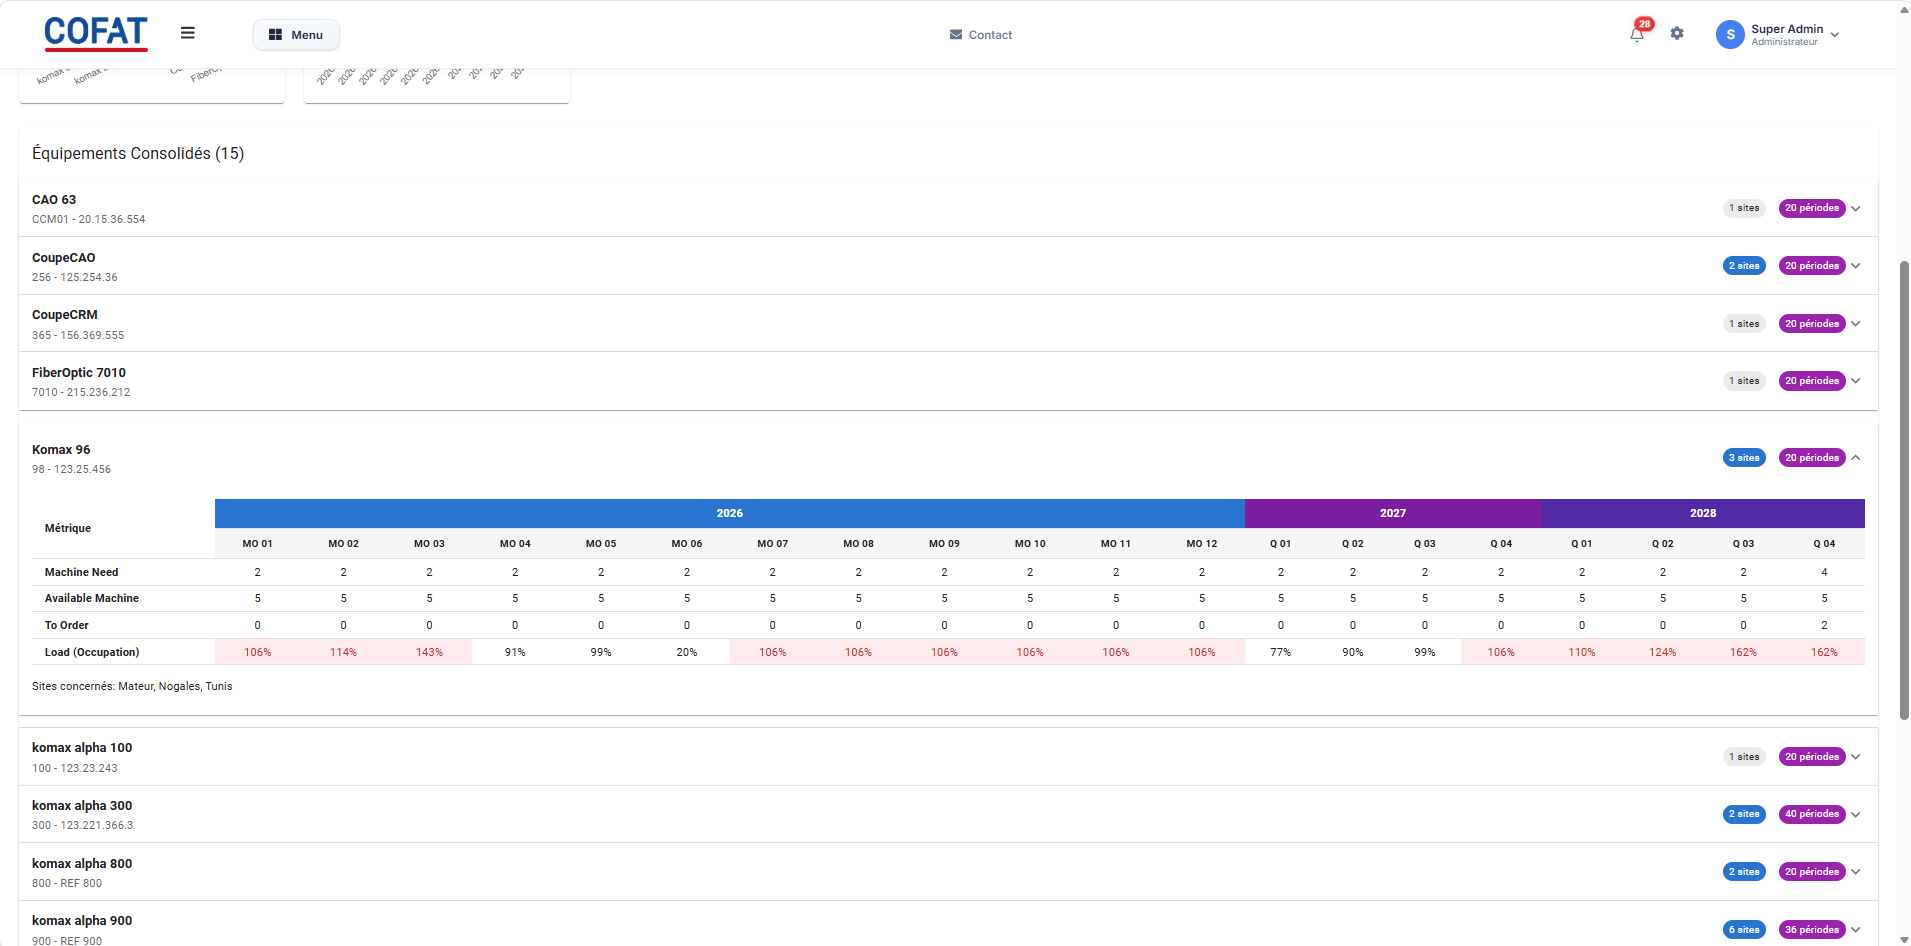
\includegraphics[width=0.9\textwidth]{img/consolidatinon cofatgroup Equipment.png}
    \caption{Tableau de consolidation mondiale des équipements industriels}
    \label{fig:conso_equipements}
\end{figure}
\vspace{0.5cm}

\textbf{L'algorithme d'agrégation (Figure \ref{fig:conso_equipements}) :}
L'API Node.js exécute une requête Sequelize utilisant les fonctions d'agrégation natives du SGBD (\texttt{sequelize.fn('SUM')}). La requête groupe les données par \textit{Type d'équipement} (\texttt{GROUP BY equipmentId}) et somme les champs \texttt{machineNeed} et \texttt{availableMachine} de \textbf{tous} les sites. 
Le résultat est éclatant pour le Backoffice : si l'usine du Mexique déclare un besoin urgent (toOrder = +2) sur une machine Komax, et que l'usine d'Égypte déclare un surplus sur ce même modèle (toOrder = -2), le tableau consolidé affichera un \textit{toOrder mondial} de zéro. La direction saura immédiatement qu'au lieu d'acheter deux machines neuves, elle doit simplement ordonner le transfert physique des machines d'Égypte vers le Mexique, économisant ainsi des centaines de milliers d'euros en une seule vue logicielle.

\subsection{Consolidation des Espaces et des RH}
Le même principe d'agrégation mathématique est appliqué aux surfaces industrielles et aux effectifs.

\vspace{0.5cm}
\begin{figure}[H]
    \centering
    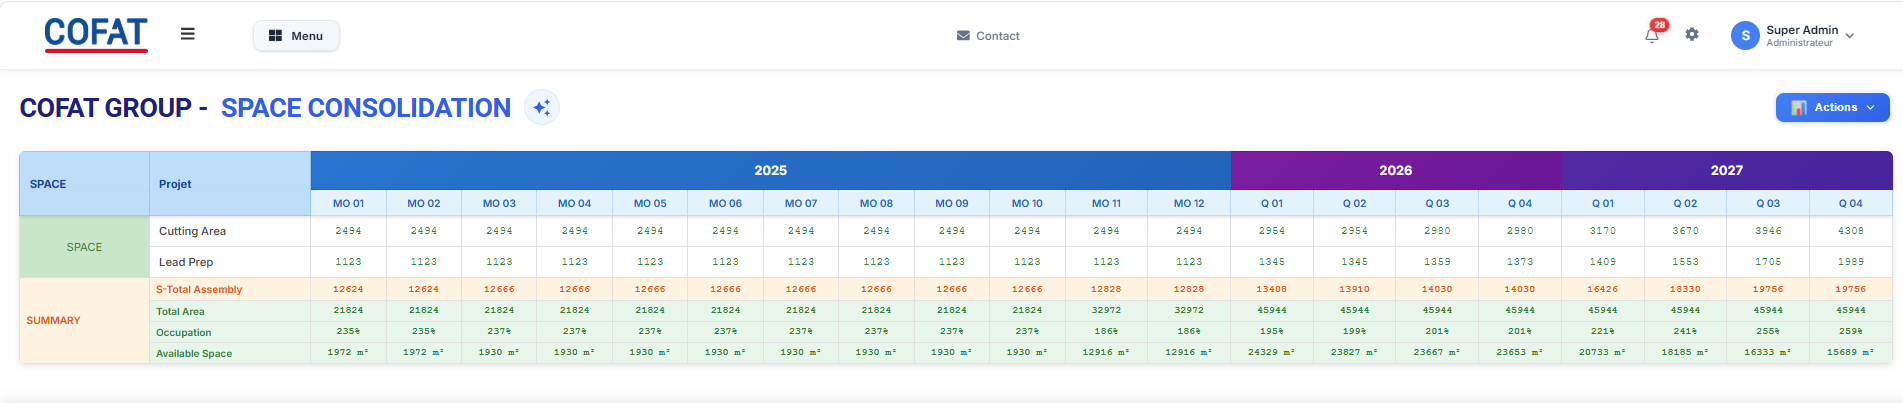
\includegraphics[width=0.9\textwidth]{img/cofat group space consolidation.png}
    \caption{Consolidation mondiale de l'occupation des usines COFAT}
    \label{fig:conso_espaces}
\end{figure}
\vspace{0.5cm}

La Figure \ref{fig:conso_espaces} montre la sommation des surfaces au sol mondiales, par typologie de zone (Coupe, Assemblage). Le graphe consolidé permet à la direction immobilière du groupe de visualiser le taux d'occupation foncier total de COFAT à travers le monde.

\vspace{0.5cm}
\begin{figure}[H]
    \centering
    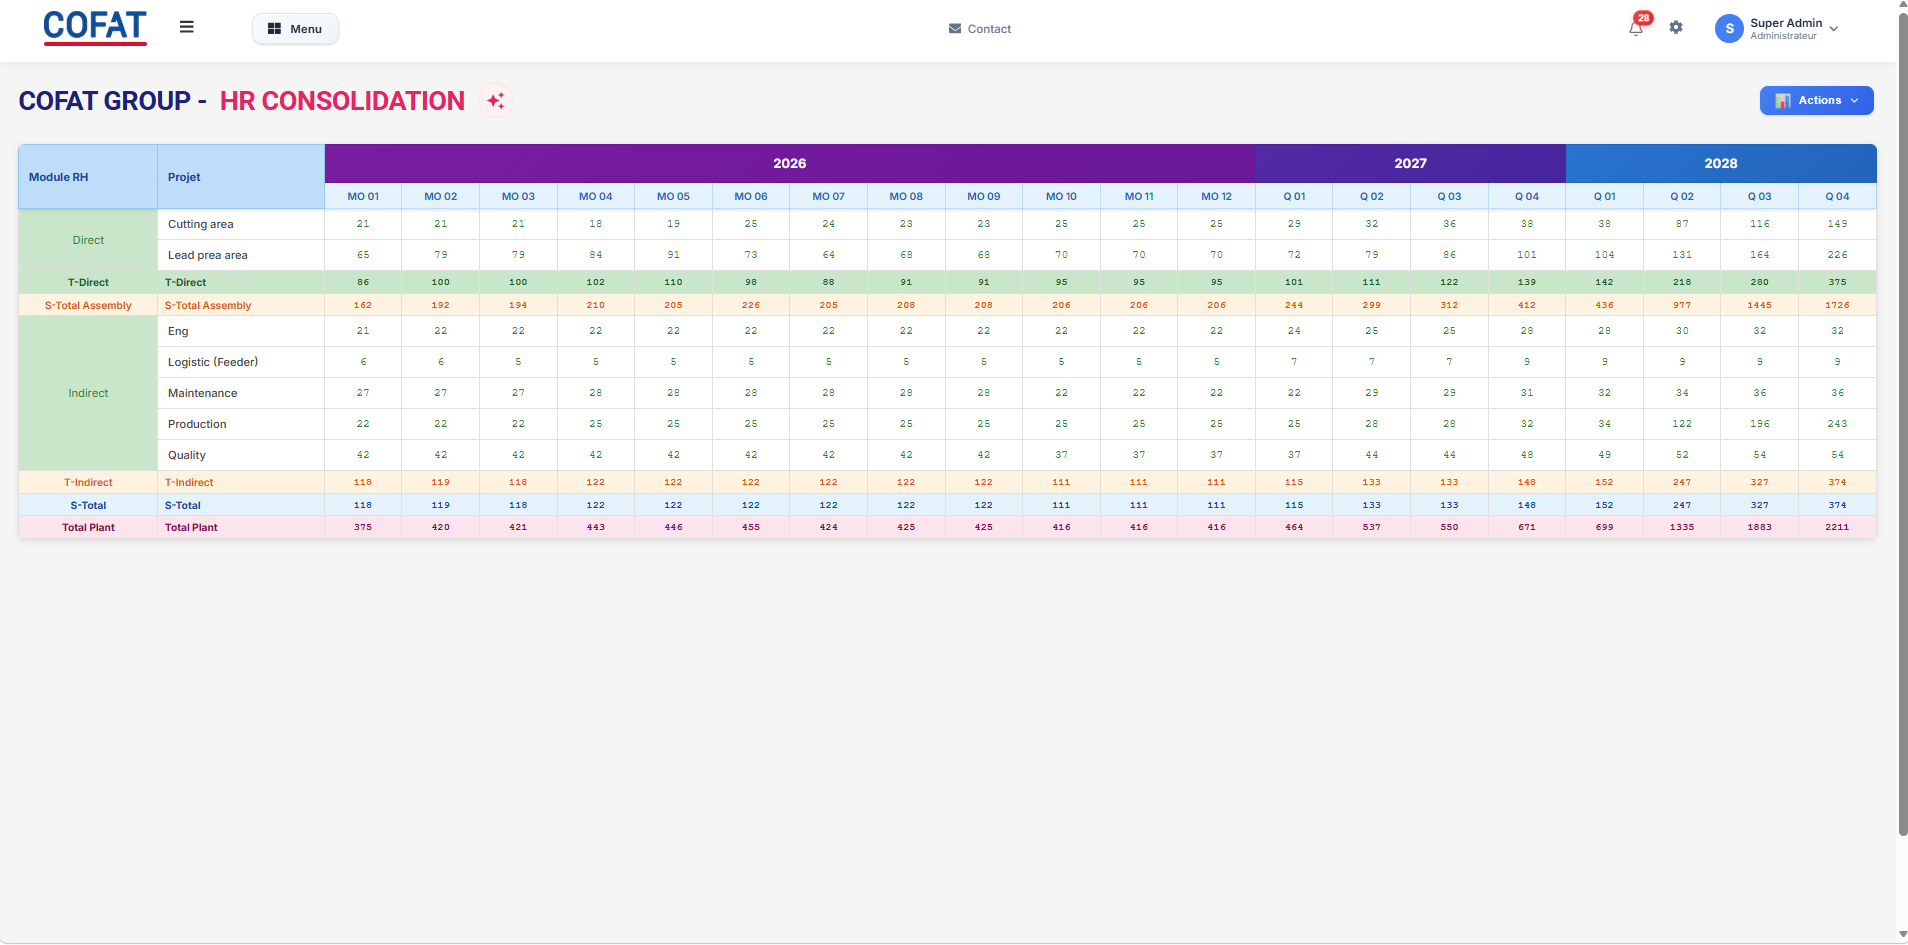
\includegraphics[width=1\textwidth]{img/cofat group HR consolidation.png}
    \caption{Tableau de consolidation RH mondial par projet et catégorie}
    \label{fig:conso_rh_table}
\end{figure}
\vspace{0.5cm}

\vspace{0.5cm}
\begin{figure}[H]
    \centering
    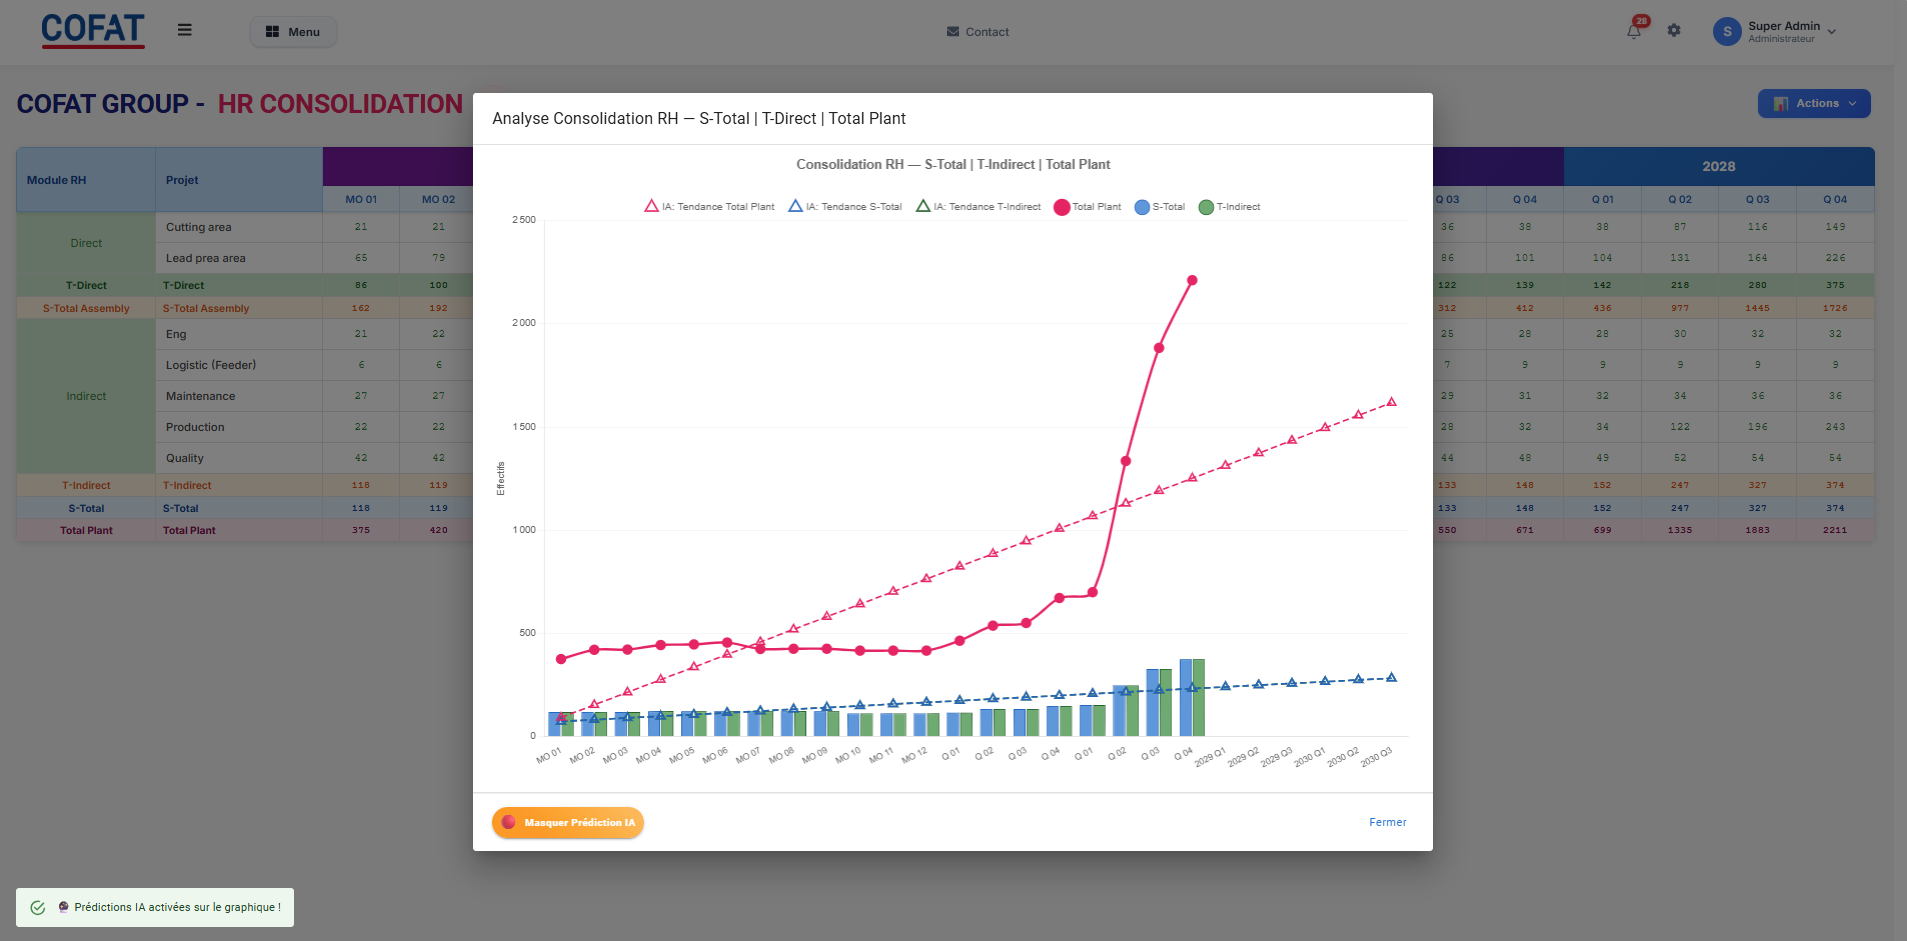
\includegraphics[width=0.9\textwidth]{img/analyse cofat group HR consolidation.png}
    \caption{Dashboard analytique de la montée en charge RH mondiale (Ramp-up)}
    \label{fig:conso_rh_graph}
\end{figure}
\vspace{0.5cm}

\textbf{Analyse de l'agrégation RH (Figures \ref{fig:conso_rh_table} et \ref{fig:conso_rh_graph}) :}
La Figure \ref{fig:conso_rh_table} affiche la somme matricielle des effectifs prévus sur 3 ans (2025-2027) pour les 5 600 employés, fusionnée à partir des 10 sites. 
Pour rendre ce mur de chiffres intelligible, l'application génère automatiquement le Dashboard analytique de la Figure \ref{fig:conso_rh_graph} via \textit{Charts.js}. Ce graphique en barres empilées par période montre l'évolution de la main-d'œuvre nécessaire (par exemple, le pic d'embauche prévu au trimestre Q02 de 2026 pour le démarrage simultané du projet VW Golf 8 en Allemagne et au Mexique). Une courbe de tendance (visible sur la capture d'écran) traverse le graphique, offrant une vision lissée de la trajectoire de recrutement global, facilitant les décisions du DRH du groupe.

\section{Le Catalogue : StandardInvestment V2}
Pour calculer les budgets nécessaires aux déficits capacitaires (\textit{toOrder}), il fallait uniformiser les bases de calcul. Si l'usine tunisienne estime une machine de coupe à 150 000 euros via un fournisseur européen, et l'usine brésilienne à 170 000 dollars via un acteur local, la consolidation financière mondiale est biaisée.
Le sprint 3 s'est donc clôturé par la réalisation du module \textit{StandardInvestment V2}, le dictionnaire mondial des prix d'équipements imposé par COFAT.

\vspace{0.5cm}
\begin{figure}[H]
    \centering
    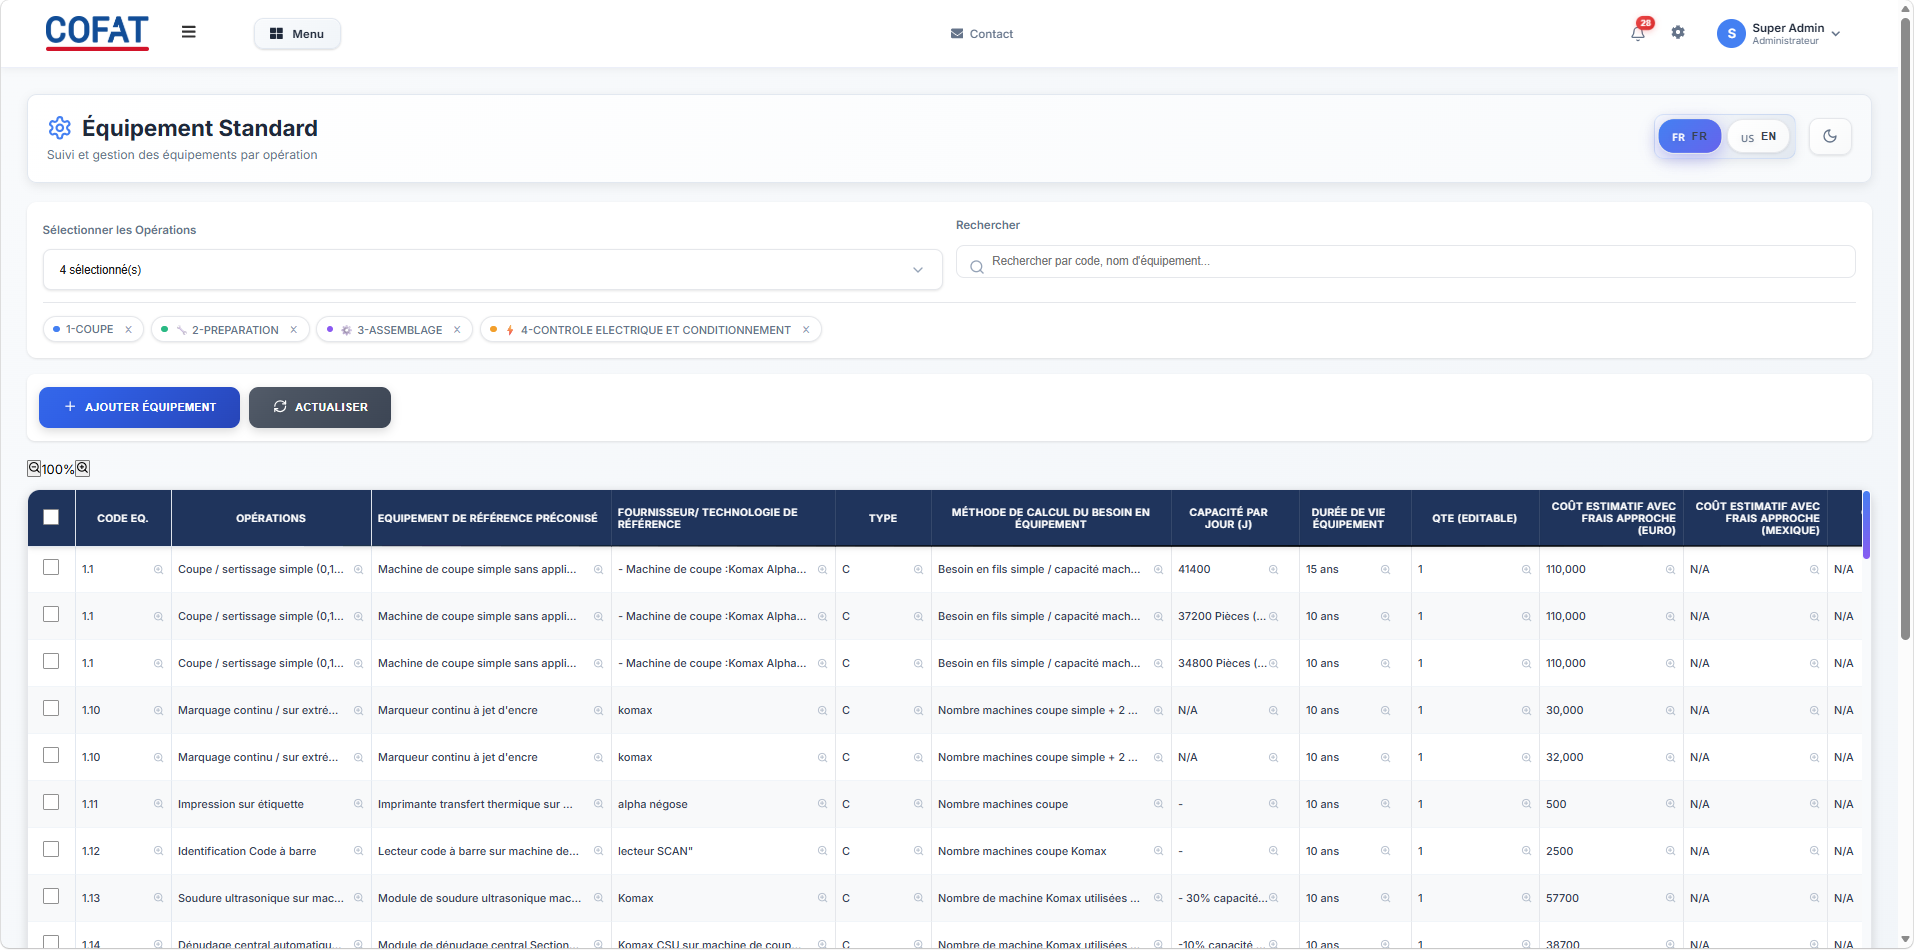
\includegraphics[width=0.9\textwidth]{img/equipement standard.png}
    \caption{Catalogue centralisé StandardInvestment V2}
    \label{fig:standard_equip}
\end{figure}
\vspace{0.5cm}

\textbf{Analyse des champs du modèle de référence (Figure \ref{fig:standard_equip}) :}
L'interface (développée avec la DataGrid de MUI) expose les champs de l'entité SQL \texttt{StandardInvestment}, listant exhaustivement les critères techniques et commerciaux obligatoires d'une machine homologuée :
\begin{itemize}
    \item \textbf{CODE EQ. et TYPE} : Identifiant unique de l'équipement dans l'ERP du groupe.
    \item \textbf{OPERATIONS} : Étape du processus (Coupe, Sertissage).
    \item \textbf{EQUIPEMENT DE REFERENCE PRECONISE} : Modèle exact de la machine (ex: Komax, Schleuniger).
    \item \textbf{FOURNISSEUR/TECHNOLOGIE DE REFERENCE} : Le partenaire industriel homologué.
    \item \textbf{CAPACITE PAR JOUR (J) et DUREE DE VIE} : Paramètres techniques pour calculer l'amortissement.
    \item \textbf{COUT ESTIMATIF AVEC FRAIS APPROCHE (EURO/MEXIQUE/...)} : Les grilles tarifaires par zone géographique.
\end{itemize}

\vspace{0.5cm}
\begin{figure}[H]
    \centering
    
\includegraphics[width=0.8\textwidth]{img/equipement standard ajout 1.png}
    \caption{Formulaire d'ajout d'un équipement standard (Partie 1)}
    \label{fig:add_standard_1}
\end{figure}
\vspace{0.5cm}

\vspace{0.5cm}
\begin{figure}[H]
    \centering
    
\includegraphics[width=0.8\textwidth]{img/equipement standard ajout 2.png}
    \caption{Formulaire d'ajout d'un équipement standard (Partie 2 : Coûts)}
    \label{fig:add_standard_2}
\end{figure}
\vspace{0.5cm}

\textbf{Gestion des Permissions : L'action de l'Acheteur (Achat) :}
Comme spécifié dans le Chapitre 2, la création (Figures \ref{fig:add_standard_1} et \ref{fig:add_standard_2}) ou la suppression de nouveaux standards est réservée à l'Administrateur central. L'Acheteur (Achat), en tant que négociateur externe, possède des droits précis sur ce catalogue : il est le garant de la justesse des prix affichés. Sa seule action sur ce module est de modifier et mettre à jour les montants dans les \textbf{trois colonnes des coûts estimatifs} : Euro (\texttt{cost\_euro}), Réal Brésilien (\texttt{cost\_brazil\_real}) et Peso Mexicain (\texttt{cost\_mexican\_peso}). Ces prix mis à jour sont ensuite utilisés par le système pour monétiser la colonne \textit{toOrder} des planifications locales. Il ne peut ni créer, ni supprimer d'équipements dans ce catalogue.

\vspace{0.5cm}
\begin{figure}[H]
    \centering
    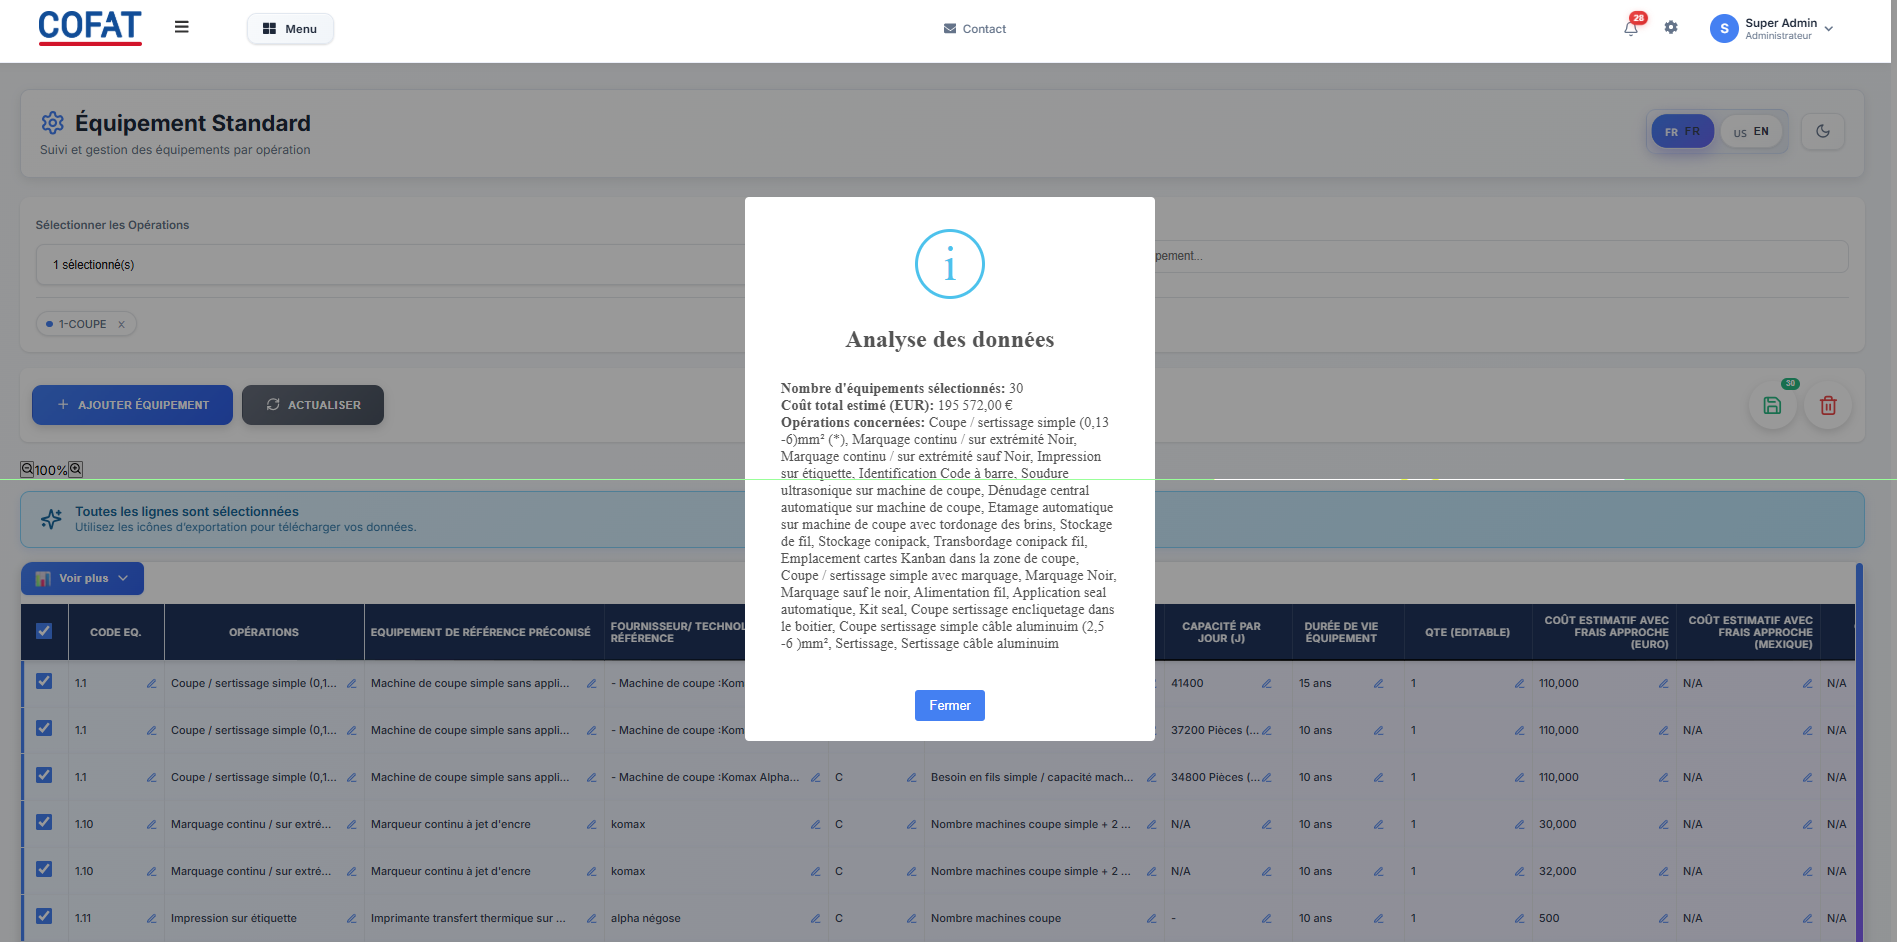
\includegraphics[width=0.9\textwidth]{img/analyse equipement standard.png}
    \caption{Analyse graphique du catalogue des équipements standards}
    \label{fig:analyse_standard}
\end{figure}
\vspace{0.5cm}

\section{Conclusion}
Les Sprints 2 et 3 ont transformé une vision théorique en un outil industriel redoutable. Le déploiement des interfaces de planification locale offre enfin aux responsables d'usine l'autonomie et la clarté nécessaires à la gestion de leurs capacités. Le développement minutieux de l'import Excel, traitant validation et injection massive (SQL bulkCreate), garantit une transition numérique sans friction pour les employés habitués aux tableurs.
En capitalisant sur cette base de données fraîchement alimentée, le moteur de consolidation mondiale (Sprint 3) délivre instantanément des tableaux de bord interactifs à la direction. Couplée à la rigueur du catalogue centralisé \textit{StandardInvestment V2}, l'application COFAT Capacity Study permet désormais d'optimiser le parc machine mondial et de prévenir les sous-charges ou surcharges d'usines.
L'étape ultime du projet, couverte par le Sprint 4 (Chapitre 5), consistera à numériser le circuit d'approbation financière à travers un workflow dynamique dédié aux budgets non-industriels.